%\bigskip
%\hrule
%\smallskip
%\hfill Edited by Takayoshi Shoudai on 2024-05-18 (2nd version), 2024-10-30 (3rd version).

\begin{lem}\label{追加部分}
  Let $\Sigma$ be an alphabet with $\sharp\Sigma \ge 3$ and $p,~q$ regular patterns on $\Sigma\cup X$.
  Let $D$ be the following set of regular patterns on $\Sigma\cup X$.
  Then, if $p \{ x := r \} \preceq q$ for all $r \in D$, then $p \{ x := xy \} \preceq q$:
  \begin{enumerate}
  \item[] $D = \{ ya, bc, dy \}$ $(b \not\in \{a,d\}$ and $c \not\in \{a,d\})$.
  \end{enumerate}
\end{lem}

  \begin{proof}
  It is obvious if no variable symbol appears in $p$.
  Thus, for a variable symbol $x\in X$, let $p=p_{1}xp_{2}$, where $p_{1}, p_{2}$ are regular patterns on $\Sigma\cup X$.
  We assume that $p \{ x := xy \} \not \preceq q$ in order to derive the contradiction.

  Since $p \{ x := r \} \preceq q$ for all $r \in D$, there are three strings of length $2$ corresponding to $ya, bc, dy$ in $q$.
  Note that the three strings may appear partly overlapping.
  The symbols appearing in $D$ corresponds to a variable or a constant in $q$.
  Let $y_{1}, y_{2}, y_{3}$ be variable symbols appearing in $q$.
  The strings $ya$ and $dy$ must correspond to the strings $y_{1}a$ and $dy_{2}$ in $q$, respectively.
  There are the following three possibilities of strings in $q$ that corresponds to $bc$ in $p\{x:=bc\}$.
  \begin{center}
    \begin{tabular}{cccccc}
      \textrm{(a)} & $bc$, & \textrm{(b)} & $y_{3}c$, & \textrm{(c)} & $by_{3}$.
    \end{tabular}
  \end{center}

  First of all, we show that the cases (b) and (c) are not possible. Suppose that there exists $y_{3}c$ in $q$ that corresponds to $bc$ in $p\{x:=bc\}$. The regular pattern $q$ can be expressed in one of the following forms:
  \begin{enumerate}
    \item[(b-1)] $q=q_{1}AwBw^{\prime}Cq_{2}$, where $\{ A,B,C \} = \{ y_{1}a, dy_{2}, y_{3}c \}$ for distinct variable symbols $y_{1}, y_{2}, y_{3}\in X$, and each of $w, w^{\prime}$ is either an empty string or a regular pattern on $\Sigma\cup X$.
    \item[(b-2)] $q=q_{1}AwBq_{2}$, where $\{ A,B \} = \{ dy_{1}a, y_{3}c \}$ for a variable symbol $y_{1}, y_{3}\in X$ and $w$ is either an empty string or a regular pattern on $\Sigma\cup X$.
    \item[(b-3)] $q=q_{1}AwBq_{2}$, where $\{ A,B \} = \{ y_{1}ay_{2}, y_{3}c \}$ ($a = d$) for distinct variable symbols $y_{1}, y_{2}\in X$, and $w$ is either an empty string or a regular pattern on $\Sigma\cup X$.
    \item[(b-4)] $q=q_{1}Aq_{2}$, where $A = y_{1}ay_{2}c$ ($a = d$) for distinct variable symbols $y_{1}, y_{2}\in X$.
  \end{enumerate}

\noindent
In the case of (b-1), suppose that $(A, B, C) = (dy_{2}, y_{1}a, y_{3}c)$, i.e., $q=q_{1}dy_{2}wy_{1}aw^{\prime}y_{3}cq_{2}$ holds.
For some $y_{1}^{\prime},y_{2}^{\prime},y_{3}^{\prime}\in X$, the following conditions hold:
\begin{align*}
  \textrm{(1)}~& p_{1} \preceq q_{1} & \textrm{(1')}~& p_{2} \preceq wy_{1}aw^{\prime}y_{3}cq_{2}, \mbox{ or} \\
      & & & p_{2} \preceq y_{2}^{\prime}wy_{1}aw^{\prime}y_{3}cq_{2}\\
  \textrm{(2)}~& p_{1} \preceq q_{1}dy_{2}w, \mbox{ or}  & \textrm{(2')}~& p_{2} \preceq w^{\prime}y_{3}cq_{2}\\
      & p_{1} \preceq q_{1}dy_{2}wy_{1}^{\prime} & & \\
  \textrm{(3)}~& p_{1} \preceq q_{1}dy_{2}wy_{1}aw^{\prime}, \mbox{ or} & \textrm{(3')}~& p_{2} \preceq q_{2}\\
      & p_{1} \preceq q_{1}dy_{2}wy_{1}aw^{\prime}y_{3}^{\prime} & &
\end{align*}
  When $p_{1} \preceq q_{1}dy_{2}wy_{1}aw^{\prime}$ of (3) and $p_{2} \preceq wy_{1}aw^{\prime}y_{3}cq_{2}$ of (1') hold, let 
  
  $q^{\prime}_{1}=q_{1}dy_{2}$, $q^{\prime}_{2}=wy_{1}aw^{\prime}$, and $q^{\prime}_{3}=y_{3}cq_{2}$.
  
  \noindent
  When $p_{1} \preceq q_{1}dy_{2}wy_{1}aw^{\prime}$ of (3) and $p_{2} \preceq y_{2}^{\prime}wy_{1}aw^{\prime}y_{3}cq_{2}$ of (1') hold, let
  
  $q^{\prime}_{1}=q_{1}d$, $q^{\prime}_{2}=y_{2}wy_{1}aw^{\prime}$, and $q^{\prime}_{3}=y_{3}cq_{2}$.
  
  \noindent
  When $p_{1} \preceq q_{1}dy_{2}wy_{1}aw^{\prime}y_{3}^{\prime}$ of (3) and $p_{2} \preceq wy_{1}aw^{\prime}y_{3}cq_{2}$ of (1') hold, let
  
  $q^{\prime}_{1}=q_{1}dy_{2}$, $q^{\prime}_{2}=wy_{1}aw^{\prime}y_{3}$, and $q^{\prime}_{3}=cq_{2}$.
  
  \noindent
  When $p_{1} \preceq q_{1}dy_{2}wy_{1}aw^{\prime}y_{3}^{\prime}$ of (3) and $p_{2} \preceq y_{2}^{\prime}wy_{1}aw^{\prime}y_{3}cq_{2}$ of (1') hold, let
  
  $q^{\prime}_{1}=q_{1}d$, $q^{\prime}_{2}=y_{2}wy_{1}aw^{\prime}y_{3}$, and $q^{\prime}_{3}=cq_{2}$.
  
  \noindent
  In any case, $p_{1} \preceq q^{\prime}_{1}q^{\prime}_{2}$ and $p_{2} \preceq q^{\prime}_{2}q^{\prime}_{3}$ hold, and $q^{\prime}_{2}$ contains at least one variable symbol. Therefore, from Theorem~\ref{Sato1:Lemma9}, $p \preceq q$ holds. It contradicts the assumption. Similarly, we can show that in every case $(A, B, C) = (y_{1}a, dy_{2}, y_{3}c)$, $(y_{3}c, y_{1}a, dy_{2})$, $(y_{3}c, dy_{2}, y_{1}a)$ of (b-1), it results in a contradiction from Theorem~\ref{Sato1:Lemma9}.

  Additionally, contradictions are derived from Theorem 2 in cases (b-2), (b-3), (b-4) and also in all cases of (c).
  From this, the cases (b) and (c) are not possible. Therefore, in the following, we consider only the case of (a).

  Since $p \{ x := xy \} \not \preceq q$, the regular pattern $q$ can be expressed in one of the following forms:
  \begin{enumerate}
  \item[(a-1)] $q=q_{1}AwBw^{\prime}Cq_{2}$, where $\{ A,B,C \} = \{ y_{1}a,bc,dy_{2} \}$ for distinct variable symbols $y_{1}, y_{2}\in X$, and each of $w, w^{\prime}$ is either an empty string or a regular pattern on $\Sigma\cup X$.
  \item[(a-2)] $q=q_{1}AwBq_{2}$, where $\{ A,B \} = \{ dy_{1}a,bc \}$ for a variable symbol $y_{1}\in X$ and $w$ is either an empty string or a regular pattern on $\Sigma\cup X$.
  \item[(a-3)] $q=q_{1}AwBq_{2}$, where $\{ A,B \} = \{ y_{1}ay_{2},bc \}$ ($a = d$) for distinct variable symbols $y_{1}, y_{2}\in X$, and $w$ is either an empty string or a regular pattern on $\Sigma\cup X$.
  \end{enumerate}
  
  Firstly, we will prove that for the case (a-1), $p \{ x := xy \} \preceq q$ holds.

  \smallskip

  \noindent
  \textit{Claim} 1. $B \not\in \{y_{1}a, dy_{2}\}$.

  \smallskip
  \noindent
  \textit{Proof of Claim} 1.
  Suppose that $(A, B, C) = (dy_{2}, y_{1}a, bc)$. For some $y_{1}^{\prime},y_{2}^{\prime}\in X$, the following conditions hold:
  \begin{align*}
    \textrm{(1)}~& p_{1} \preceq q_{1} & \textrm{(1')}~& p_{2} \preceq wy_{1}aw^{\prime}bcq_{2}, \mbox{ or} \\
    & & & p_{2} \preceq y_{2}^{\prime}wy_{1}aw^{\prime}bcq_{2}\\
    \textrm{(2)}~& p_{1} \preceq q_{1}dy_{2}w, \mbox{ or}  & \textrm{(2')}~& p_{2} \preceq w^{\prime}bcq_{2}\\
    & p_{1} \preceq q_{1}dy_{2}wy_{1}^{\prime} & & \\
    \textrm{(3)}~& p_{1} \preceq q_{1}dy_{2}wy_{1}aw^{\prime} & \textrm{(3')}~& p_{2} \preceq q_{2}
  \end{align*}
  When $p_{2} \preceq wy_{1}aw^{\prime}bcq_{2}$ of (1') holds, let $q^{\prime}_{1}=q_{1}dy_{2},~q^{\prime}_{2}=wy_{1}aw^{\prime},~q^{\prime}_{3}=bcq_{2}$. Since $p_{1} \preceq q_{1}dy_{2}wy_{1}aw^{\prime}$ holds from (3), $p_{1} \preceq q^{\prime}_{1}q^{\prime}_{2}$ and $p_{2} \preceq q^{\prime}_{2}q^{\prime}_{3}$ hold and $q_{2}^{\prime}$ contains a variable symbol.
  %
  When $p_{2} \preceq y_{2}^{\prime}wy_{1}aw^{\prime}bcq_{2}$ of (1') holds, let $q^{\prime}_{1}=q_{1}d,~q^{\prime}_{2}=y_{2}wy_{1}aw^{\prime},~q^{\prime}_{3}=bcq_{2}$. Since $p_{1} \preceq q_{1}dy_{2}wy_{1}aw^{\prime}$ holds from (3), $p_{1} \preceq q^{\prime}_{1}q^{\prime}_{2}$ and $p_{2} \preceq q^{\prime}_{2}q^{\prime}_{3}$ hold and $q_{2}^{\prime}$ contains a variable symbol.
  In both cases, from Theorem~\ref{Sato1:Lemma9}, $p \preceq q$ holds. It contradicts the assumption.

  Similarly, we can show that any case of $(A, B, C) = (y_{1}a, dy_{2}, bc)$, $(bc, y_{1}a, dy_{2})$, $(bc, dy_{2}, y_{1}a)$ contradicts the assumption.
  %
  Therefore, we have $B \not\in \{y_{1}a, dy_{2}\}$. (\textit{End of Proof of Claim})

  \smallskip

  \noindent
  \textit{Claim} 2. $(A, B, C) = (y_{1}a, bc, dy_{2})$.

  \smallskip
  \noindent
  \textit{Proof of Claim} 2.
  From \textit{Claim} 1, we have $B=bc$. Suppose that $(A, B, C) = (dy_{2}, bc, y_{1}a)$, i.e., $q = q_{1}dy_{2}wbcw^{\prime}y_{1}aq_{2} $ holds. Then, the following conditions hold: for $y_{1}^{\prime},y_{2}^{\prime}\in X$,
  \begin{align*}
  \textrm{(1)}~& p_{1} \preceq q_{1} & \textrm{(1')}~& p_{2} \preceq wbcw^{\prime}y_{1}aq_{2}, \mbox{ or}\\
  & & & p_{2} \preceq y_{2}^{\prime}wbcw^{\prime}y_{1}aq_{2}\\
  \textrm{(2)}~& p_{1} \preceq q_{1}dy_{2}w & \textrm{(2')}~& p_{2} \preceq w^{\prime}y_{1}aq_{2} \\
  \textrm{(3)}~& p_{1} \preceq q_{1}dy_{2}wbcw^{\prime}, \mbox{ or} & \textrm{(3')}~& p_{2} \preceq q_{2}\\
  & p_{1} \preceq q_{1}dy_{2}wbcw^{\prime}y_{1}^{\prime}& &
  \end{align*}
  %
  %When $p_{1} \preceq q_{1}dy_{2}wbcw^{\prime}y_{1}^{\prime}$ of (3) and $p_{2} \preceq y_{2}^{\prime}wbcw^{\prime}y_{1}aq_{2}$ of (1') hold, let $q^{\prime}_{1}=q_{1}d,~q^{\prime}_{2}=y_{2}wbcw^{\prime}y_{1},~q^{\prime}_{3}=aq_{2}$.
  %
  %When $p_{1} \preceq q_{1}dy_{2}wbcw^{\prime}$ of (3) and $p_{2} \preceq y_{2}^{\prime}wbcw^{\prime}y_{1}aq_{2}$ of (1') hold, let $q^{\prime}_{1}=q_{1}d$, $q^{\prime}_{2}=y_{2}wbcw^{\prime}$, $q^{\prime}_{3}=y_{1}aq_{2}$.
  %
  %When $p_{1} \preceq q_{1}dy_{2}wbcw^{\prime}y_{1}^{\prime}$ of (3) and $p_{2} \preceq wbcw^{\prime}y_{1}aq_{2}$ of (1') hold, let $q^{\prime}_{1}=q_{1}dy_{2}$, $q^{\prime}_{2}=wbcw^{\prime}y_{1}$, $q^{\prime}_{3}=aq_{2}$. 
  %
  %These imply $p_{1} \preceq q^{\prime}_{1}q^{\prime}_{2}$, $p_{2} \preceq q^{\prime}_{2}q^{\prime}_{3}$, and $q_{2}^{\prime}$ contains a variable symbol. In these three cases, from Theorem~\ref{Sato1:Lemma9}, $p \preceq q$ holds. It contradicts the assumption.
  %
  %We suppose that $p_{2} \preceq wbcw^{\prime}y_{1}aq_{2}$ of (1') hold.
  From $p_{1} \preceq q_{1}dy_{2}w$ of (2), for some $p^{\prime}_{1}$ and $p^{\prime\prime}_{1}$, $p_{1}$ is expressed as $p^{\prime}_{1}p^{\prime\prime}_{1}$, where $p^{\prime}_{1} \preceq q_{1}d$ and $p^{\prime\prime}_{1} \preceq y_{2}w$. 
  When $p_{2} \preceq wbcw^{\prime}y_{1}aq_{2}$ of (1'), we have $p=p_{1}xp_{2}=p^{\prime}_{1}p^{\prime\prime}_{1}xp_{2} \preceq q_{1}dp^{\prime\prime}_{1}xwbcw^{\prime}y_{1}aq_{2}=q \{ y_{2}:=p^{\prime\prime}_{1}x \}$. Thus, $p \{ x := xy \} \preceq q \{ y_{2}:=p^{\prime\prime}_{1}xy \}$ holds. It contradicts the assumption.
  %
  When $p_{2} \preceq y_{2}^{\prime}wbcw^{\prime}y_{1}aq_{2}$ of (1'), we have $p=p_{1}xp_{2}=p^{\prime}_{1}p^{\prime\prime}_{1}xp_{2} \preceq q_{1}dp^{\prime\prime}_{1}xy_{2}^{\prime}wbcw^{\prime}y_{1}aq_{2}=q \{ y_{2}:=p^{\prime\prime}_{1}xy_{2}^{\prime} \}$.
  Thus, $p \{ x := xy \} \preceq q \{ y_{2}:=p^{\prime\prime}_{1}xyy_{2}^{\prime} \}$ holds. It contradicts the assumption.
  %
  Therefore, we have $(A, B, C) = (y_{1}a, bc, dy_{2})$.
  (\textit{End of Proof of Claim})

  \smallskip

  From \textit{Claim} 2, $q$ is expressed as $q_{1}y_{1}awbcw^{\prime}dy_{2}q_{2}$, where $b \not\in \{a,d\}$ and $c \not\in \{a,d\}$.
  If $p \{ x := xy \} \not \preceq q$ holds, we have the following conditions:
  for $y_{1}^{\prime},y_{2}^{\prime}\in X$,
  \begin{align*}
    \textrm{(1)}~& p_{1} \preceq q_{1} \mbox{ or} p_{1} \preceq q_{1}y_{1}^{\prime} & \textrm{(1')}~& p_{2} \preceq wbcw^{\prime}dy_{2}q_{2} \\
    \textrm{(2)}~& p_{1} \preceq q_{1}y_{1}aw & \textrm{(2')}~& p_{2} \preceq w^{\prime}dy_{2}q_{2} \\
    \textrm{(3)}~& p_{1} \preceq q_{1}y_{1}awbcw^{\prime} & \textrm{(3')}~& p_{2} \preceq q_{2} \mbox{ or} p_{2} \preceq y_{2}^{\prime}q_{2}
  \end{align*}

  \smallskip

  \noindent
  \textit{Claim} 3. $w$ and $w'$ contains no variable symbol.

  \smallskip
  \noindent
  \textit{Proof of Claim} 3.
  Let $q_{1}^{\prime} = q_{1}y_{1}a$, $q_{2}^{\prime} = wbcw^{\prime}$, and $q_{3}^{\prime} = dy_{2}q_{2}$. From (1') and (3), $p_{1} \preceq q^{\prime}_{1}q^{\prime}_{2}$ and $p_{2} \preceq q^{\prime}_{2}q^{\prime}_{3}$. If $q_{2}^{\prime}$ contains a variable symbol, from Theorem~\ref{Sato1:Lemma9}, $p \preceq q$ holds. It contradicts the assumption. Therefore, $w$ and $w'$ contains no variable symbol. (\textit{End of Proof of Claim})

  \smallskip

  From \textit{Claim} 3, $w$ and $w'$ are strings consisting of symbols in $\Sigma$. Note that from (1') and (2'), $wbcw^{\prime}d$ and $w^{\prime}d$ are prefixes of $p_{2}$, and from (2) and (3), $awbcw^{\prime}$ and $aw$ are suffixes of $p_{1}$.

  If $|w|=|w^{\prime}|$, then $c=a$ holds.
  It contradicts the condition $c \not = a$.
  
  If $|w|=|w^{\prime}|+1$, then $b = a$ holds.
  It contradicts the condition $b \not = a$.
  
  If $|w| = |w^{\prime}|+2$, since $awbcw^{\prime}$ and $aw$ are suffixes of $p_{1}$, and since $|w|\geq 2$, $a$ is a suffix of $w$.
  From (1') and (2'), since $wbcw^{\prime}d$ and $w^{\prime}d$ are prefixes of $p_{2}$, we have $w=w^{\prime}da$.
  Since $awbcw^{\prime}$ and $aw$ are suffixes of $p_{1}$, we have $w=bcw^{\prime}$.
  Therefore, $w^{\prime}da = bcw^{\prime}$ holds. We show the next claim:

  \smallskip

  \noindent
  \textit{Claim} 4.
  Let $w^{\prime}$ be a string of constant symbols in $\Sigma$ and $a,b,c,d$ constant symbols in $\Sigma$.
  Then, if $b \not\in \{a,d\}$ and $c \not\in \{a,d\}$, then $w^{\prime}da \not = bcw^{\prime}$ holds.
  %\end{cl}

  \smallskip
  
  \noindent
  \textit{Proof of Claim} 4.
  When $|w^{\prime}| = 0, 1, 2, 3$, it is easy to see that $w^{\prime}da=bcw^{\prime}$ does not satisfy the conditions $b \not\in \{a,d\}$ and $c \not\in \{a,d\}$. Therefore, $w^{\prime}da \not= bcw^{\prime}$ holds.
  Let $n = |w^{\prime}|$.
  When $n \ge 4$, we assume that for any string $w^{\prime\prime}$ with $|w^{\prime\prime}|<n$, if $b \not\in \{a,d\}$ and $c \not\in \{a,d\}$, $w^{\prime\prime}da \not =bcw^{\prime\prime}$ holds.
  Since the string $w^{\prime}$ has a prefix $bc$ and a suffix $da$, there exists a string $w^{\prime\prime}$ with $|w^{\prime\prime}| \geq 0$ such that $w^{\prime}=bcw^{\prime\prime}da$ holds.
  Since $w^{\prime}da=bcw^{\prime\prime}dada$ and $bcw^{\prime}=bcbcw^{\prime\prime}da$, if $w^{\prime}da = bcw^{\prime}$ holds, we have $bcw^{\prime\prime}dada=bcbcw^{\prime\prime}da$.
  Then we conclude that $w^{\prime\prime}da=bcw^{\prime\prime}$.
  It contradicts the induction hypothesis. Thus, $w^{\prime}da \not= bcw^{\prime}$ holds.
  From the above, for any string $w^{\prime}$ with $|w^{\prime}| \geq 0$, if $b \not\in \{a,d\}$ and $c \not\in \{a,d\}$, $w^{\prime}da \not =bcw^{\prime}$ holds.
  (\textit{End of Proof of Claim})
  
  \smallskip

  \noindent
  Thus, the case of $|w|=|w^{\prime}|+2$ contradicts \textit{Claim} 4. 

  If $|w| \ge |w^{\prime}|+3$, from (2) and (3), there exists a string $w^{\prime\prime}$ of length $|w|-|w^{\prime}|-2$ such that $w=w^{\prime\prime}bcw^{\prime}$ holds.
  Moreover, from (2) and (3), since $|aw| < |wbcw^{\prime}|$ and $aw = aw^{\prime\prime}bcw^{\prime}$, $aw^{\prime\prime}$ is a suffix of $w$.
  On the other hand, from (1') and (2'), $w^{\prime}d$ is a prefix of $w$.
  Since $|w^{\prime}d| + |aw^{\prime\prime}| = |w^{\prime}| + |w^{\prime\prime}| + 2 = |w|$, we have $w=w^{\prime}daw^{\prime\prime}$.
  Therefore, $w^{\prime}daw^{\prime\prime} = w^{\prime\prime}bcw^{\prime}$ holds.
  
  \smallskip
  
  \noindent
  \textit{Claim} 5.
  Let $w^{\prime},w^{\prime\prime}$ be strings of constant symbols in $\Sigma$ and $a,b,c,d$ constant symbols in $\Sigma$.
  Then, if $b \not\in \{a,d\}$ and $c \not\in \{a,d\}$, then $w^{\prime}daw^{\prime\prime} \not = w^{\prime\prime}bcw^{\prime}$ holds.

  \smallskip
  
  \noindent
  \textit{Proof of Claim} 5.
  We assume that the following equation holds:
  \begin{equation}
  w^{\prime}daw^{\prime\prime} = w^{\prime\prime}bcw^{\prime}\label{eq:claim2}
  \end{equation}
  We prove this claim by an induction on $|w^{\prime}| + |w^{\prime\prime}|$.
  W.l.o.g., we suppose that $|w^{\prime}| \geq |w^{\prime\prime}|$ holds.
  \begin{enumerate}
    \item[(i)] $|w^{\prime}| \geq 0$ and $|w^{\prime\prime}|=0$:
    We have $w^{\prime}da = bcw^{\prime}$ ($b \not\in \{a,d\}$ and $c \not\in \{a,d\}$).
    It contradicts \textit{Claim} 4.
  \end{enumerate}
  We assume that for constant strings $u$ and $v$ with $|u| + |v| < |w^{\prime}| + |w^{\prime\prime}|$, $vbcu \not= udav$ holds.
  We partition the relations between $|w^{\prime}|$ and $|w^{\prime\prime}|$ into the following four parts:
  \begin{enumerate}
  \item[(ii)] $0 < |w^{\prime\prime}| \le |w^{\prime}| \le |w^{\prime\prime}|+1$:
  When either $|w^{\prime}|=|w^{\prime\prime}|$ or $|w^{\prime}|=|w^{\prime\prime}|+1$, Eq.~\ref{eq:claim2} is depicted as shown in Figs.~\ref{追加部分7}, \ref{追加部分8}. Trivially, these cases contradict the conditions $b \not\in \{a,d\}$ and $c \not\in \{a,d\}$.
  %When $|w^{\prime}|=|w^{\prime\prime}|+2$, Eq.~\ref{eq:claim2} can be written as shown in Fig.~\ref{追加部分9}. This implies $w^{\prime}=w^{\prime\prime}bc=daw^{\prime\prime}$, and then contradicts \textit{Claim} 1.
  \item[(iii)] $|w^{\prime\prime}|+2 \le |w^{\prime}| \le 2|w^{\prime\prime}| - 1$:
  On Eq.~\ref{eq:claim2}, since $|w^{\prime}daw^{\prime\prime}| = |w^{\prime\prime}bcw^{\prime}| = |w^{\prime}| + |w^{\prime\prime}| + 2$, a suffix of $w^{\prime}$ overlaps with a prefix of $w^{\prime}$ as shown in Fig.~\ref{w1+3}. That is, there exists a constant string $u$ of length $2|w^{\prime}| - (|w^{\prime}| + |w^{\prime\prime}| + 2) = |w^{\prime}| - |w^{\prime\prime}| - 2$ such that $u$ is a prefix and a suffix of $w^{\prime}$.
  Since $uda$ is of length $|w^{\prime}| - |w^{\prime\prime}|$, $uda$ is also a prefix of $w^{\prime}$. Similarly, $bcu$ is also a suffix of $w^{\prime}$.
  Since $|w^{\prime}| - (|uda| + |bcu|) = 2|w^{\prime\prime}| - |w^{\prime}| \ge 1$, there exist a constant string $v$ of length $2|w^{\prime\prime}| - |w^{\prime}|$ such that $w^{\prime} = udavbcu$ holds. Since $w^{\prime\prime}$ is a suffix of $w^{\prime}$ and $|vbcu| = (2|w^{\prime\prime}| - |w^{\prime}|) + 2 + (|w^{\prime}| - |w^{\prime\prime}| - 2) = |w^{\prime\prime}|$, we have $w^{\prime\prime} = vbcu$. Similarly, we have $w^{\prime\prime} = udav$. Thus, we have a new equation $vbcu = udav$.
  Since $|u| = |w^{\prime}| - |w^{\prime\prime}| - 2 \leq |w^{\prime\prime}| - 3 < |w^{\prime\prime}|$ and $|v| = 2|w^{\prime\prime}| - |w^{\prime}| < |w^{\prime}|$, i.e., $|u| + |v| < |w^{\prime}| + |w^{\prime\prime}|$ holds, it contradicts the induction hypothesis on $|u| + |v|$. Therefore, the claim holds.
  \item[(iv)] $2|w^{\prime\prime}| \le |w^{\prime}| \le 2|w^{\prime\prime}|+3$:
  When $|w^{\prime}|=2|w^{\prime\prime}|$, we easily see that $w^{\prime} = w^{\prime\prime}w^{\prime\prime}$.
  Therefore, $w^{\prime\prime}da = bcw^{\prime\prime}$ holds as shown in Fig.~\ref{追加部分14}.
  It contradicts \textit{Claim} 3.
  When $|w^{\prime}|=2|w^{\prime\prime}|+i$ ($i=1,2,3$), Eq.~\ref{eq:claim2} is depicted as shown in Figs.~\ref{追加部分13}, \ref{追加部分12}, and \ref{追加部分11}. Trivially, these cases contradict the conditions $b \not\in \{a,d\}$ and $c \not\in \{a,d\}$.
  \item[(v)] $2|w^{\prime\prime}|+4 \leq |w^{\prime}|$:
  Since the strings $w^{\prime\prime}bc$ and $adw^{\prime\prime}$ are a prefix and a suffix of $w^{\prime}$, respectively, and $|w^{\prime\prime}bc| + |adw^{\prime\prime}| = 2|w^{\prime\prime}| + 4$, there exists a string $u$ with $|u| \geq 0$ such that $w^{\prime} = w^{\prime\prime}bcudaw^{\prime\prime}$ holds. From Eq.~\ref{eq:claim2}, $w^{\prime\prime}bcudaw^{\prime\prime}daw^{\prime\prime} = w^{\prime\prime}bcw^{\prime\prime}bcudaw^{\prime\prime}$, i.e., $udaw^{\prime\prime} = w^{\prime\prime}bcu$ holds as shown in Fig.~\ref{2w1+5}.
  Let $v = w^{\prime\prime}$.
  Since $|u| + |v| = |w^{\prime}|- (2|w^{\prime\prime}| + 4) + |w^{\prime\prime}| < |w^{\prime}| + |w^{\prime\prime}|$, it contradicts the induction hypothesis on $|u| + |v|$. Therefore, the claim holds.
  \end{enumerate}
  From the above, we conclude that $w^{\prime}daw^{\prime\prime} \not = w^{\prime\prime}bcw^{\prime}$ holds.
  (\textit{End of Proof of Claim})

\smallskip

\noindent
Thus, the case of $|w| \geq |w^{\prime}| + 3$ contradicts \textit{Claim} 5. 

\begin{figure}[t]
  \begin{center}
    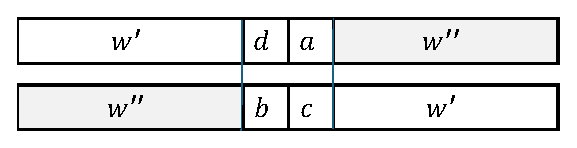
\includegraphics[scale=0.45]{figs/w=w_1.eps}
    \caption{Subcase $|w^{\prime}| = |w^{\prime\prime}|$ of (ii) of \textit{Claim} 5 (Lemma~\ref{追加部分})}\label{追加部分7}
    \bigskip
    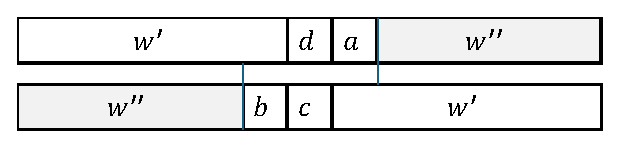
\includegraphics[scale=0.45]{figs/w=w_1+1.eps}
    \caption{Subcase $|w^{\prime}| = |w^{\prime\prime}| + 1$ of (ii) of \textit{Claim} 5 (Lemma~\ref{追加部分})}\label{追加部分8}
    %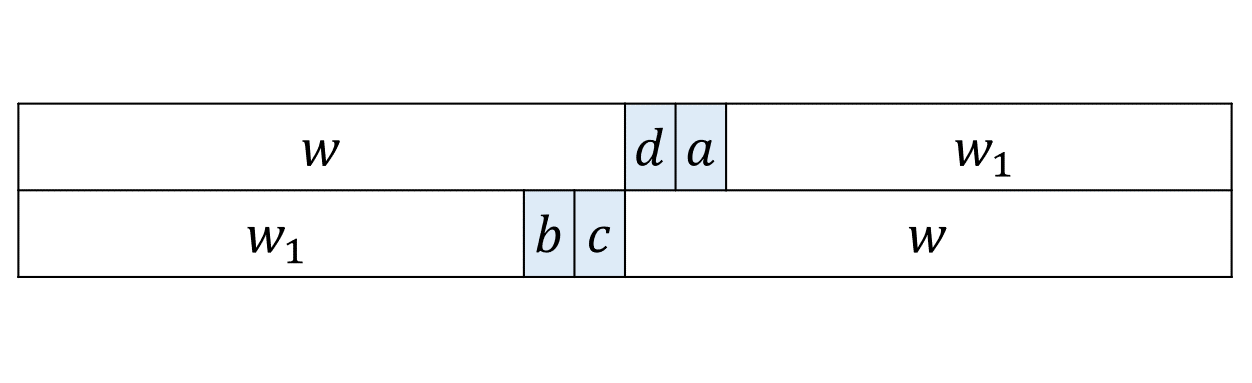
\includegraphics[scale=0.35]{figs/w=w_1+2.png}
    %\caption{Subcase $|w^{\prime}| = |w^{\prime\prime}| + 2$ of (ii) of \textit{Claim} 5 (Lemma~\ref{追加部分})}\label{追加部分9}
  \end{center}
\end{figure}

\begin{figure}[t]
  \begin{center}
    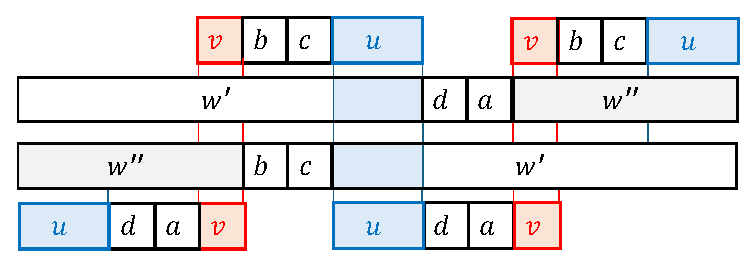
\includegraphics[scale=0.45]{figs/w=w_1+2.eps}
    \caption{Case $|w^{\prime\prime}| + 2 \le |w^{\prime}| \le 2|w^{\prime\prime}| - 1$ of (iii) of \textit{Claim} 5 (Lemma~\ref{追加部分})}\label{w1+3}
  \end{center}
\end{figure}

\begin{figure}[t]
  \begin{center}
    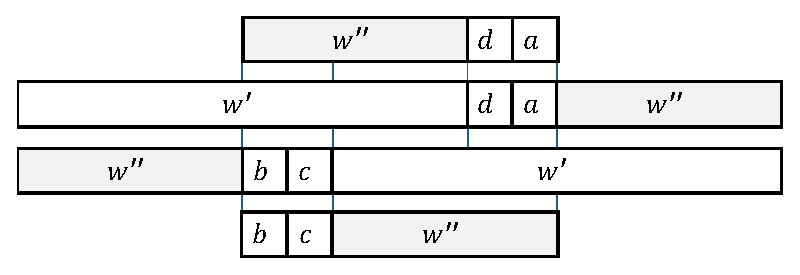
\includegraphics[scale=0.45]{figs/w=2w_1.eps}
    \caption{Subcase $|w^{\prime}| = 2|w^{\prime\prime}|$ of (iv) of \textit{Claim} 5 (Lemma~\ref{追加部分})}\label{追加部分14}
    \bigskip
    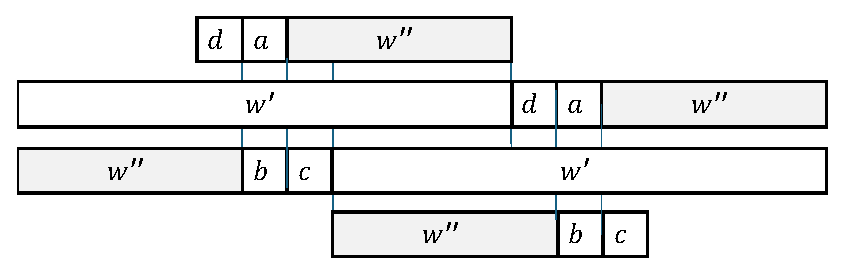
\includegraphics[scale=0.45]{figs/w=2w_1+1.eps}
    \caption{Subcase $|w^{\prime}| = 2|w^{\prime\prime}| + 1$ of (iv) of \textit{Claim} 5 (Lemma~\ref{追加部分})}\label{追加部分13}
    \bigskip
    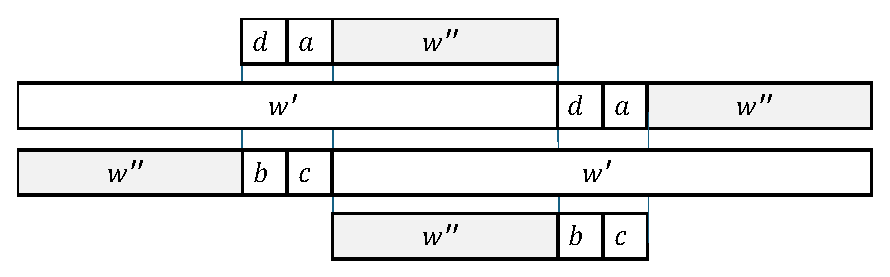
\includegraphics[scale=0.45]{figs/w=2w_1+2.eps}
    \caption{Subcase $|w^{\prime}| = 2|w^{\prime\prime}| + 2$ of (iv) of \textit{Claim} 5 (Lemma~\ref{追加部分})}\label{追加部分12}
    \bigskip
    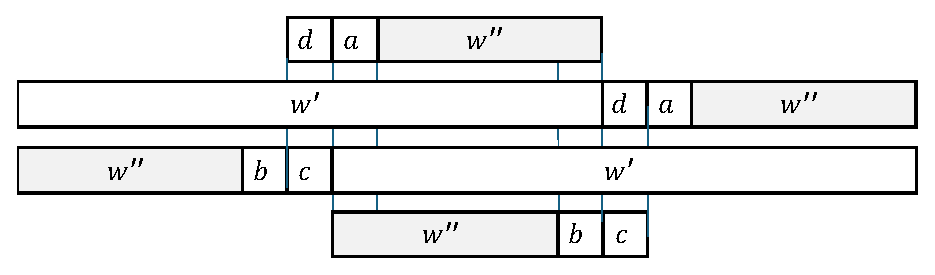
\includegraphics[scale=0.45]{figs/w=2w_1+3.eps}
    \caption{Subcase $|w^{\prime}| = 2|w^{\prime\prime}| + 3$ of (iv) of \textit{Claim} 5 (Lemma~\ref{追加部分})}\label{追加部分11}
    %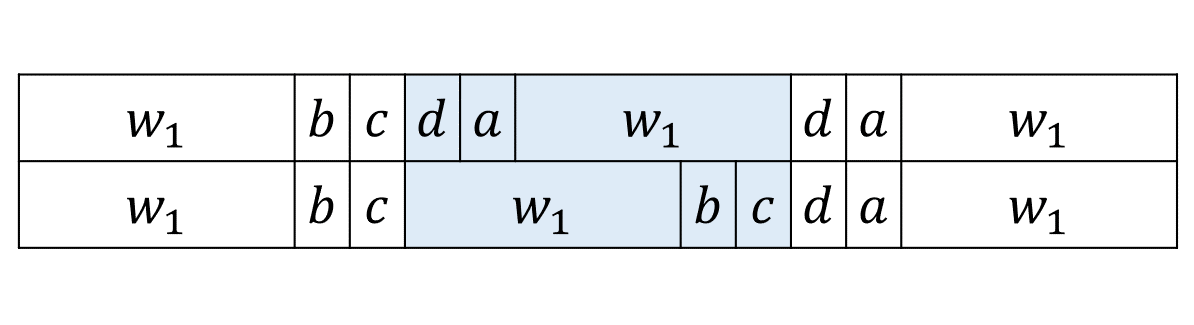
\includegraphics[scale=0.35]{figs/w=2w_1+4.png}
    %\caption{$|w| = 2|w_{1}|+4$における定数記号列}\label{追加部分10}
  \end{center}
\end{figure}

\begin{figure}[t]
  \begin{center}
    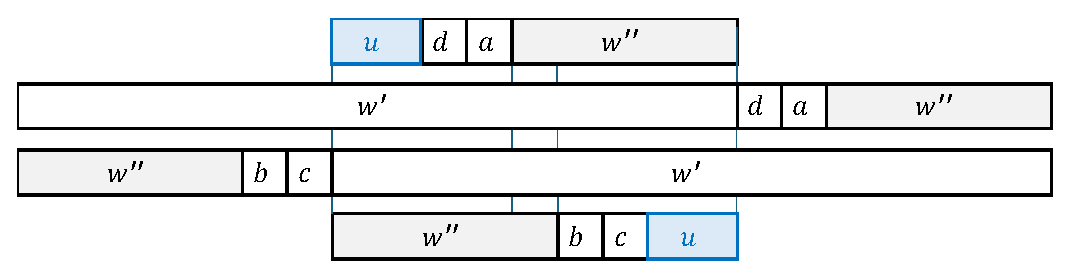
\includegraphics[scale=0.45]{figs/w=2w_1+4.eps}
    \caption{Case $2|w^{\prime\prime}| + 4 \leq |w^{\prime}|$ of (v) of \textit{Claim} 5 (Lemma~\ref{追加部分})}\label{2w1+5}
  \end{center}
\end{figure}
    
  Next, we suppose that $|w| < |w^{\prime}|$ holds.
  Note again that from (1') and (2'), $wbcw^{\prime}d$ and $w^{\prime}d$ are prefixes of $p_{2}$, and from (2) and (3), $awbcw^{\prime}$ and $aw$ are suffixes of $p_{1}$.
  
  If $|w^{\prime}|=|w|+1$, since $|wbc|=|w^{\prime}d|$, we have $c=d$. This contradicts the condition $c \ne d$.
  
  If $|w^{\prime}|=|w|+2$, since $|wbc|=|w^{\prime}|$, $bc$ is a suffix of $w^{\prime}$.
  Moreover, since $w^{\prime}d$ is a prefix of $wbcw^{\prime}$, $d$ is the first symbol of $w^{\prime}$.
  Since $aw$ is a suffix of $w'$ and $|w^{\prime}|=|aw|+1$, $a$ is the second symbol of $w^{\prime}$.
  Therefore, we have $w^{\prime}=wbc=daw$.
  This contradicts \textit{Claim} 4.
  
  If $|w^{\prime}| \ge |w|+3$, there exists a string $w^{\prime\prime}$ with $|w^{\prime\prime}| \geq 1$ such that $w^{\prime} = wbcw^{\prime\prime}$ holds.
  Then, since $wbcw^{\prime}d$ and $w^{\prime}d=wbcw^{\prime\prime}d$ are prefixes of $p_{2}$, $w^{\prime\prime}d$ is a prefix of $w^{\prime}$.
  Since $w^{\prime}$ and $aw$ are suffixes of $p_{1}$ and $|w^{\prime}|=|wbcw^{\prime\prime}|=|w|+|w^{\prime\prime}|+2 > |aw|$, $aw$ is a suffix of $w^{\prime}$.
  Since $|w^{\prime\prime}d| + |aw| = |w^{\prime}|$, we have $w^{\prime} = w^{\prime\prime}daw$.
  Therefore, we have $w^{\prime}=wbcw^{\prime\prime}=w^{\prime\prime}daw$.
  This contradicts \textit{Claim} 5.

  Thus, the case $(A, B, C) = (y_{1}a, bc, dy_{2})$ implies the contradictions.
  
  Secondly, we will prove that for the case (a-2), $p \{ x := xy \} \preceq q$ holds. Suppose that $(A, B) = (dy_{1}a, bc)$, i.e., $q = q_{1}dy_{1}awbcq_{2} $ holds. Then, the following conditions hold: for $y_{1}^{\prime}\in X$,
  \begin{align*}
    \textrm{(1)}~& p_{1} \preceq q_{1} & \textrm{(1')}~& p_{2} \preceq awbcq_{2}, \mbox{ or} \\
    & & & p_{2} \preceq y_{1}^{\prime}awbcq_{2}\\
    \textrm{(2)}~& p_{1} \preceq q_{1}d, \mbox{ or}  & \textrm{(2')}~& p_{2} \preceq wbcq_{2}\\
    & p_{1} \preceq q_{1}dy_{1}^{\prime} & & \\
    \textrm{(3)}~& p_{1} \preceq q_{1}dy_{1}aw & \textrm{(3')}~& p_{2} \preceq q_{2}
  \end{align*}
  %
  From $p_{1} \preceq q_{1}dy_{1}aw$ of (3), for some $p^{\prime}_{1}$ and $p^{\prime\prime}_{1}$, $p_{1}$ is expressed as $p^{\prime}_{1}p^{\prime\prime}_{1}$, where $p^{\prime}_{1} \preceq q_{1}d$ and $p^{\prime\prime}_{1} \preceq y_{1}aw$. 
  When $p_{2} \preceq awbcq_{2}$ of (1'), we have $p=p_{1}xp_{2}=p^{\prime}_{1}p^{\prime\prime}_{1}xp_{2} \preceq q_{1}dp^{\prime\prime}_{1}xawbcq_{2}=q \{ y_{1}:=p^{\prime\prime}_{1}x \}$.
  Thus, $p \{ x := xy \} \preceq q \{ y_{1}:=p^{\prime\prime}_{1}xy \}$ holds. It contradicts the assumption.
  When $p_{2} \preceq y_{1}^{\prime}awbcq_{2}$ of (1'), we have $p=p_{1}xp_{2}=p^{\prime}_{1}p^{\prime\prime}_{1}xp_{2} \preceq q_{1}dp^{\prime\prime}_{1}xy_{1}^{\prime}wbcq_{2}=q \{ y_{1}:=p^{\prime\prime}_{1}xy_{1}^{\prime} \}$.
  Thus, $p \{ x := xy \} \preceq q \{ y_{1}:=p^{\prime\prime}_{1}xyy_{1}^{\prime} \}$ holds. It contradicts the assumption.
  %
  Similarly, we can show that the case $(A, B) = (bc, dy_{1}a)$ contradicts the assumption.
  
  Finally, we will prove that for the case (a-3), $p \{ x := xy \} \preceq q$ holds. Suppose that $(A, B) = (y_{1}ay_{2}, bc)$, i.e., $q = q_{1}y_{1}ay_{2}wbcq_{2} $ holds. Then, the following conditions hold: for $y_{1}^{\prime}\in X$,
  \begin{align*}
    \textrm{(1)}~& p_{1} \preceq q_{1}, \mbox{ or} & \textrm{(1')}~& p_{2} \preceq y_{2}wbcq_{2} \\
    & p_{1} \preceq q_{1}y_{1}^{\prime} & & \\
    \textrm{(2)}~& p_{1} \preceq q_{1}dy_{1} & \textrm{(2')}~& p_{2} \preceq wbcq_{2}, \mbox{ or}\\    
    & & & p_{2} \preceq y_{2}^{\prime}wbcq_{2} \\
    \textrm{(3)}~& p_{1} \preceq q_{1}y_{1}ay_{2}w & \textrm{(3')}~& p_{2} \preceq q_{2}
  \end{align*}
  %
  Let $q^{\prime}_{1}=q_{1}y_{1}a,~q^{\prime}_{2}=y_{2}w,~q^{\prime}_{3}=bcq_{2}$. From (3) and (1'), we have $p_{1} \preceq q^{\prime}_{1}q^{\prime}_{2}$ and $p_{2} \preceq q^{\prime}_{2}q^{\prime}_{3}$, respectively. Since $q_{2}^{\prime}$ contains a variable symbol,
  from Theorem~\ref{Sato1:Lemma9}, $p \preceq q$ holds. It contradicts the assumption.
  %
  Similarly, we can show that the case $(A, B) = (bc, y_{1}ay_{2})$ contradicts the assumption.
  
  \smallskip
  
  From the above, we conclude that if $p \{ x := r \} \preceq q$ for all $r = \{ ya, bc, dy \}$ $(b \not\in \{a,d\}$ and $c \not\in \{a,d\})$, then $p \{ x := xy \} \preceq q$ holds.
  \end{proof}

% To position the next figure optimally in the paper, it is placed here. (by Takayoshi Shoudai)
\begin{figure*}[t]
  %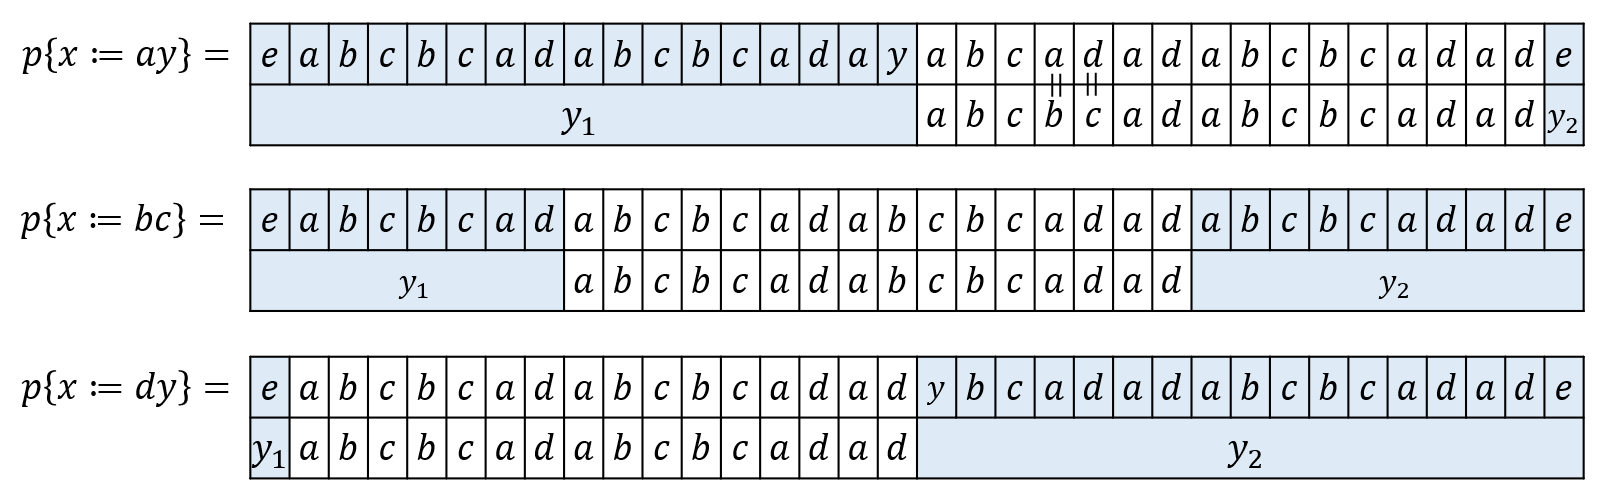
\includegraphics[width=\linewidth]{figs/Exam_b=a_c=d.png}
  \begin{center}
  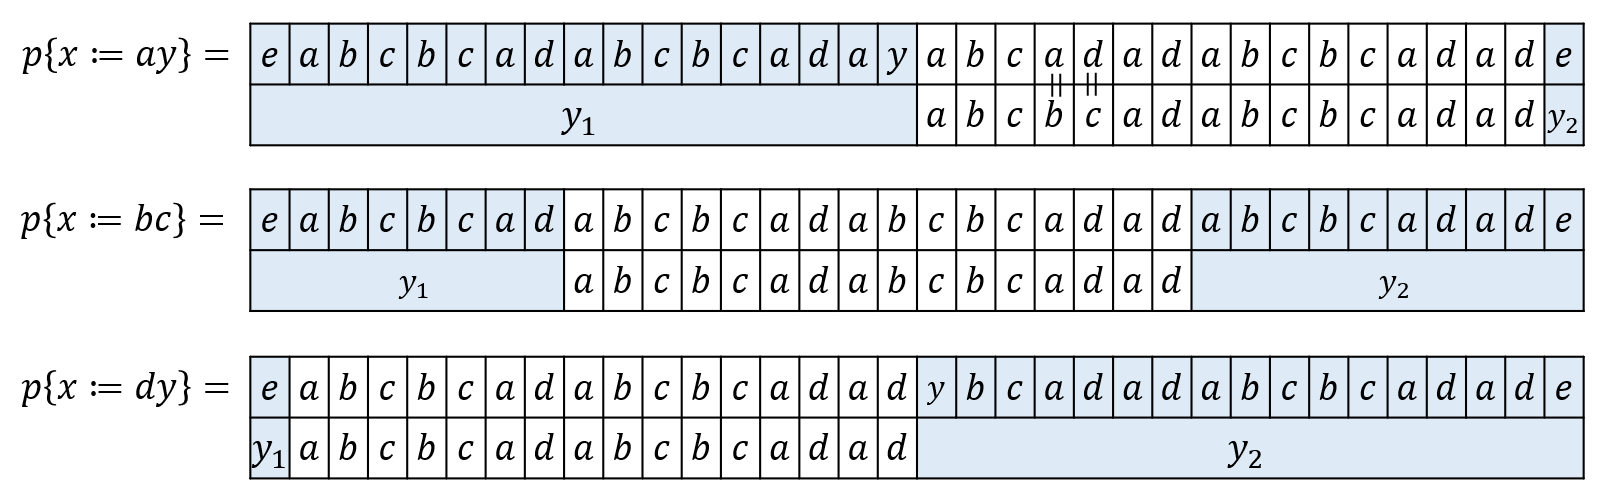
\includegraphics[scale=0.45]{figs/Exam_b=a_c=d.png}
  \end{center}
  \caption{Substitutions for $p$ and each correspondence to $q$.}
  \label{b=aとc=dの例}
\end{figure*}

\begin{lem}\label{片方}
Let $\Sigma$ be an alphabet with $\sharp\Sigma \ge 3$ and $p,~q$ regular patterns on $\Sigma\cup X$.
Let $D$ be one of the following sets \textrm{(i), (ii)} of regular patterns on $\Sigma\cup X$.
Then, if $p \{ x := r \} \preceq q$ for all $r \in D$, then $p \{ x := xy \} \preceq q$:
\begin{enumerate}
\item[{\rm (i)}] $D=\{ ya, bc, dy \}$ ($b = a,~b \not= d,\mbox{~and~}c \not\in \{a,d\}$),
\item[{\rm (ii)}] $D=\{ ya, bc, dy \}$ ($b \not\in \{a,d\},~c = d,\mbox{~and~} c \not = a$).
\end{enumerate}
\end{lem}

\begin{proof}
  It is obvious if no variable symbol appears in $p$.
  Therefore, let $p=p_{1}xp_{2}$, where $p_{1}, p_{2}$ are regular patterns and $x$ is a variable symbol. We assume that $p \{ x := xy \} \not \preceq q$ in order to derive the contradiction.
  
\noindent\textrm{(i)}
Let $D=\{ ya, bc, dy \}$ ($b = a,~b \not= d,\mbox{~and~}c \not\in \{a,d\}$).
Since $p \{ x := r \} \preceq q$ for all $r \in D$, there are three strings of length $2$ corresponding to $ya, bc, dy$ in $q$. Note that the three strings may appear partly overlapping.
The symbols appearing in $D$ corresponds to a variable or a constant in $q$.
Let $y_{1}, y_{2}, y_{3}$ be variable symbols appearing in $q$.
The strings $ya$ and $dy$ must correspond to the strings $y_{1}a$ and $dy_{3}$ in $q$, respectively.
There are the following three possibilities of strings in $q$ which corresponds to $bc$ in $p\{x:=bc\}$.
\begin{center}
\begin{tabular}{cccccc}
\textrm{(a)} & $bc$, &
\textrm{(b)} & $y_{2}c$, &
\textrm{(c)} & $by_{2}$.
\end{tabular}
\end{center}

\textrm{(a)}
Let $A,B,C$ be strings where $\{ A,B,C \} = \{ y_{1}a,bc,dy_{3} \}$ and let $q=q_{1}AwBw^{\prime}Cq_{2}$.
Since $p \{ x := r \} \preceq q$ for all $r \in D$ and $p \{ x := xy \} \not \preceq q$ hold, the following conditions hold:
\begin{align*}
  \textrm{(1)}~& p_{1} \preceq q_{1} & \textrm{(1')}~& p_{2} \preceq wBw^{\prime}Cq_{2} \\
  \textrm{(2)}~& p_{1} \preceq q_{1}Aw & \textrm{(2')}~& p_{2} \preceq w^{\prime}Cq_{2} \\
  \textrm{(3)}~& p_{1} \preceq q_{1}AwBw^{\prime} & \textrm{(3')}~& p_{2} \preceq q_{2}
\end{align*}

Let $q^{\prime}_{1}=q_{1}A,~q^{\prime}_{2}=wBw^{\prime},~q^{\prime}_{3}=Cq_{2}$.
From (3) and (1'), we have $p_{1} \preceq q^{\prime}_{1}q^{\prime}_{2},~p_{2} \preceq q^{\prime}_{2}q^{\prime}_{3}$.
From Lemma \ref{Sato1:Lemma9}, if $q^{\prime}_{2}$ contains a variable, $p \preceq q$ holds.
Therefore, $B$ must be $bc$.
If $A=dy_{3}$, from $(2)$, $p_{1} \preceq q_{1}dy_{3}w$ holds.
Let $p_{1}=p^{\prime}_{1}p^{\prime\prime}_{1}, p^{\prime}_{1} \preceq q_{1}d$, and $p^{\prime\prime}_{1} \preceq y_{3}w$.
From (1'), we have $p=p_{1}xp_{2}=p^{\prime}_{1}p^{\prime\prime}_{1}xp_{2} \preceq q_{1}dp^{\prime\prime}_{1}xwbcw^{\prime}y_{1}aq_{2}=q \{ x:=p^{\prime\prime}_{1}x \}$. This shows that there is a substitution $\theta$ such that $p=q\theta$ holds, and this contradicts the assumption. Therefore, we only need to consider the case where $A=y_{1}a,B=bc$, and $C=dy_{3}$.

From the above, we consider two cases: one in which the symbols overlap and the other in which they do not.
\smallskip

\begin{tabular}{cl}
\textrm{(a-1)} & $q=q_{1}y_{1}awbcw^{\prime}dy_{3}q_{2}$,\\
\textrm{(a-2)} & $q=q_{1}y_{1}acwdy_{3}q_{2}$~~($a=b$).
\end{tabular}
\smallskip

\textrm{(a-1)}
From the proof of Lemma \ref{追加部分}, $p \{ x:= xy \} \preceq q$ holds.
Therefore, it contradicts the assumption.

\textrm{(a-2)}
Let $q=q_{1}y_{1}acwdy_{3}q_{2}$ ($a=b$).
For this $q$, the following conditions hold:
\begin{align*}
  \textrm{(1)}~& p_{1} \preceq q_{1} & \textrm{(1')}~& p_{2} \preceq cwdy_{3}q_{2} \\
  \textrm{(2)}~& p_{1} \preceq q_{1}y_{1} & \textrm{(2')}~& p_{2} \preceq wdy_{3}q_{2} \\
  \textrm{(3)}~& p_{1} \preceq q_{1}y_{1}acwdy_{3} & \textrm{(3')}~& p_{2} \preceq q_{2}
\end{align*}

%
If $|w|=0$, from (1') and (2'), the prefix of $p_{2}$ is $cd$ and $d$.
Therefore, $c=d$. This contradicts the fact that $c \not = d$.

If $|w|=1$, from (1') and (2'), the prefix of $p_{2}$ is $cwd$ and $wd$.
Therefore, $w=c=d$.
This contradicts the fact that $c \not = d$.

If $|w| \ge 2$, then from (1') and (2'),  prefixes of $p_{2}$ is $cwd$ and $wd$.
Let $w$ be $w_{1}w_{2}w_{3} \cdots w_{n-1}w_{n}$ $(n\geq 2,~w_{i}\in\Sigma$ for $i=1, \ldots , n)$.
From $cw=wd$, a prefix of $w$ is $c$ and a suffix of $w$ is $d$.
Therefore, we have $w=cw_{2}w_{3} \cdots w_{n-1}d$.
Since $cw=cw_{2}w_{3} \cdots w_{n-1}d,~wd=cw_{2}w_{3} \cdots w_{n-1}dd$, from $cw=wd$, $w_{i}=w_{i+1}$ holds for $i=2, \ldots , n-2$.
Therefore, $c=d$. This contradicts the fact that $c \not = d$.

\textrm{(b)}
Let $q=q_{1}AwBw^{\prime}Cq_{2}$ where $\{ A,B,C \} = \{ y_{1}a,y_{2}c,dy_{3} \}$, and let $q=q_{1}AwBw^{\prime}Cq_{2}$.
Since $c \not = a$ holds, $q$ have a substring that is corresponding to (i-2) of Lemma~\ref{変数2つ}.
Therefore, $p \{ x:= xy \} \preceq q$ holds.
This contradicts the assumption. 

\textrm{(c)} As in (b), this contradicts the assumption.

\noindent\textrm{(ii)}
In this case, by reversing the strings $p$ and $q$, we can prove that the assumption $p \{ x := xy \} \preceq q$ is contradicted, as in the case of \textrm{(i)}.
\end{proof}
When the conditions of both Lemmas \ref{追加部分} and \ref{片方} are not satisfied, counterexamples exist as follows:

\newtheorem{prop}{Proposition}

\begin{prop}\label{両方}
  Let $\Sigma$ be an alphabet with $\sharp \Sigma \ge 3$.
  For a variable symbol $y$, let $D= \{ ya, bc, dy \}$ $(b = a$ and $c = d)$. There exist regular patterns $p$ and $q$ on $\Sigma$ such that $p \{ x := r \} \preceq q$ for any $r \in D$, but $p \{ x := xy \} \not \preceq q$.
\end{prop}

\begin{proof}
We give an example which shows this proposition.
Let $a,b,c,d,e$ be constant symbols in $\Sigma$ and 
$x,y,y_{1},y_{2}$ variable symbols in $X$.
Let 
\begin{align*}
p &= eabcbcadabcbcadaxbcadadabcbcadade,\\
q &= y_{1}abcbcadabcbcadady_{2}~~~~~(b = a\mbox{~and~}c = d).
\end{align*}

\noindent
Obviously $p \{ x:=xy \} \not \preceq q$ holds.
For these $p$ and $q$, the condition for Proposition~\ref{両方} holds as follows (see also Fig.~\ref{b=aとc=dの例}):
\begin{eqnarray*}
&p& \{ x:=ya \} \\ 
& = & (eabcbcadabcbcaday)abcadadabcbcadade\\
& = & q \{ y_{1} := eabcbcadabcbcaday,~y_{2}:=e \} \\
& \preceq & q,\\
&p& \{ x:=bc \}  \\
& = & (eabcbcad)abcbcadabcbcadad(abcbcadade) \\
& = & q \{ y_{1} := eabcbcad,~y_{2} := abcbcadade \} \\
& \preceq & q,\\
&p& \{ x:=dy \}  \\
& = & eabcbcadabcbcadad(ybcadadabcbcadade) \\
& = & q \{ y_{1}:=e,~y_{2} := ybcadadabcbcadade \} \\
& \preceq & q.
\end{eqnarray*}
\end{proof}

\begin{figure*}[t]
  \begin{center}
    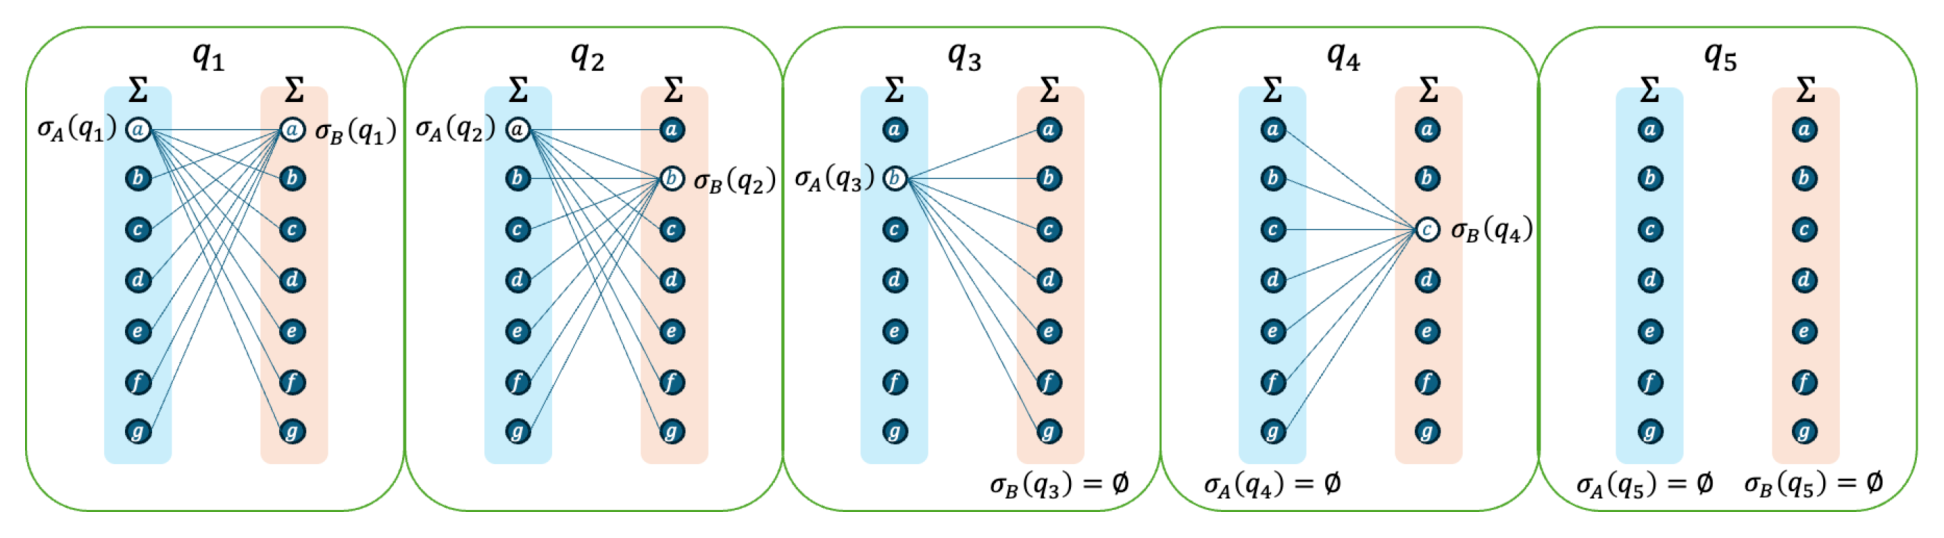
\includegraphics[scale=0.5]{figs/lem8eachreg.eps}
    \caption{Let $\Sigma=\{a,b,c,d,e,f,g\}, Q=\{q_1,q_2,q_3,q_4,q_5\}$. We set $A(q_1)=\{a\}$ and $B(q_1)=\{a\}$, and then $\sigma_A(q_1)=a$ and $\sigma_B(q_1)=a$, and so on. For each regular pattern $q_i$ ($i=1,\ldots,5$), we represent a string $w \in \Sigma\cdot\Sigma$ satisfying that $p\{x:=w\}\preceq q_i$ by the line between the left (first) and right (second) symbols of $w$. For example, the leftmost figure shows that $p\{x:=ay\}\preceq q_1$ and $p\{x:=ya\}\preceq q_1$ for a variable symbol $y$. We note that these figures may contain more lines than those depicted. From these figures, we get $\ell_A=1, \ell_B=0$, and $Q^{(\varnothing,\varnothing)}=\{q_5\}, Q^{(\varnothing,\cdot)}=\{q_4\}, Q^{(\cdot,\varnothing)}=\{q_3\}, Q^{(\cdot,\cdot)}=\{q_1,q_2\}$.}\label{fig:lem8eachreg}
  \end{center}
\end{figure*}

\begin{figure}[t]
  \begin{center}
    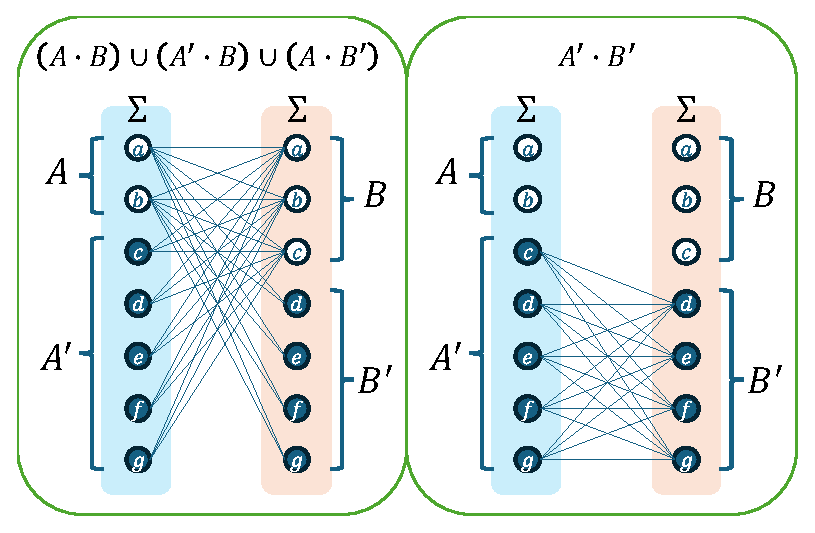
\includegraphics[scale=0.5]{figs/lem8totalreg.eps}
    \caption{In the left figure, we aggregate all of the lines appearing in Fig.~\ref{fig:lem8eachreg}. For all $w=a'b'\in A'\cdot B'$, there must be a regular pattern $q_i$ $(1\leq i\leq 5$) that satisfies that $p \{ x:=w \} \preceq q_i$.}\label{fig:lem8totalreg}
  \end{center}
\end{figure}

\begin{lem}\label{追加補題1}
Let $k$ be an integer with $k\geq 1$.
Let $\Sigma$ be an alphabet with $\sharp \Sigma = k + 2$.
Let $p \in \RPat$ in which a variable symbol $x$ appears, and let $Q \in \RPat^{k}$.
If for any string $w \in \Sigma^{\ast}$ with $|w|=2$, there exists a regular pattern $q_{w} \in Q$ such that $p \{ x:=w \} \preceq q_{w}$ holds, then there exists a regular pattern $q \in Q$ such that $p \{ x:=xy \} \preceq q$ holds, where $y$ is a variable symbol that does not appear in $q$.
\end{lem}

\begin{proof}
W.l.o.g., we suppose that $\sharp Q = k$ holds. Otherwise, for some regular pattern $q$ already in $Q$, we can add a new regular pattern $q'$ equivalent to $q$, i.e., $q' \equiv q$, to $Q$ repeatedly until $\sharp Q = k$ is satisfied.
For any $q \in Q$, we define the sets $A(q), B(q) \subseteq \Sigma$ as follows:
\begin{align*}
  A(q) & = \{ a \in \Sigma \mid p \{ x:=ay \} \preceq q,\ y\in X\},\\ 
  B(q) & = \{ b \in \Sigma \mid p \{ x:=yb \} \preceq q,\ y\in X\}.
  \end{align*}
If there exists $q\in Q$ such that $|A(q)|\geq 2$ or $|B(q)|\geq 2$, from Lemma~\ref{変数2つ}, $p\{x := xy\} \preceq q$ holds.
Below, we suppose that $|A(q)|\leq 1$ and $|B(q)|\leq 1$.
Let $\varnothing$ be a constant symbol that is not a member in $\Sigma$.
We define the functions $\sigma_{A}: Q \rightarrow \Sigma \cup \{\varnothing\}$ and $\sigma_{B}: Q \rightarrow \Sigma \cup \{\varnothing\}$ as follows:
\begin{align*}
  \sigma_{A}(q) & =
  \begin{cases}
    a & \textrm{if } A(q) = \{a\}, \\
    \varnothing & \textrm{if } A(q) = \emptyset.
  \end{cases}\\
  \sigma_{B}(q) & =
  \begin{cases}
    b & \textrm{if } B(q) = \{b\}, \\
    \varnothing & \textrm{if } B(q) = \emptyset.
  \end{cases}
\end{align*}
The inverse functions of $\sigma_{A}$ and $\sigma_{B}$ are denoted by $\sigma_{A}^{-1}$ and $\sigma_{B}^{-1}$, respectively. That is, for $a,b \in \Sigma \cup \{\varnothing\}$, let $\sigma_{A}^{-1}(a) = \{q \in Q \mid \sigma_{A}(q) = a\}$ and $\sigma_{B}^{-1}(b) = \{q \in Q \mid \sigma_{B}(q) = b\}$. 
We give an example in Fig.~\ref{fig:lem8eachreg}.

$A$ and $B$ denotes the following subsets of $\Sigma$:
\begin{align*}
  A & = \bigcup_{q \in Q \setminus \sigma_{A}^{-1}(\varnothing)} A(q) \mbox{,~~~}
  B = \bigcup_{q \in Q \setminus \sigma_{B}^{-1}(\varnothing)} B(q).
\end{align*}
Then, let $A' = \Sigma \setminus A$ and $B' = \Sigma \setminus B$.
For any $a,b \in \Sigma$, we use the following notations:
\begin{align*}
  %\ell_{A}(a) & = \{ q \in Q \mid p \{ x:=ay \} \preceq q,\ y\in X\},\\ 
  %\ell_{B}(b) & = \{ q \in Q \mid p \{ x:=yb \} \preceq q,\ y\in X\}\\
  %\ell_{A} &= \sum_{a \in \Sigma}(\ell_{A}(a) - 1),\\
  \ell_{A} &= \sum_{a \in A}(\sharp \sigma_{A}^{-1}(a) - 1) \mbox{,~~~}
  %\ell_{B} &= \sum_{b\in \Sigma}(\ell_{B}(b) - 1).
  \ell_{B} = \sum_{b \in B}(\sharp \sigma_{B}^{-1}(b) - 1).
\end{align*}
These $\ell_{A}$ and $\ell_{B}$ represent the numbers of excess duplicate symbols in $A$ and $B$.
We easily see the following claim:  

\smallskip

\noindent
\textit{Claim} 1. 
\begin{enumerate}
  \item[(i)] $\sharp A + \sharp A' = \sharp B + \sharp B' = k + 2$,
  \item[(ii)] $\sharp A + \ell_{A} + \sharp \sigma_{A}^{-1}(\varnothing) = \sharp B + \ell_{B} + \sharp \sigma_{B}^{-1}(\varnothing) = k$.
\end{enumerate}

\smallskip

Since $\sharp \Sigma = k + 2$ and $\sharp Q = k$, $\sharp A' \geq 2$ and $\sharp B' \geq 2$ hold.
We partition $Q$ into the following subsets:
\begin{align*}
  %Q^{(\varnothing,\varnothing)} & = \{q \in Q \mid \sigma_{A}(q) = \varnothing \textrm{~and~} \sigma_{B}(q) = \varnothing\},\\
  Q^{(\varnothing,\varnothing)} & = \sigma_{A}^{-1}(\varnothing) \cap \sigma_{B}^{-1}(\varnothing),\\
  %Q^{(\varnothing,\cdot)} & = \{q \in Q \mid \sigma_{A}(q) = \varnothing \textrm{~and~} \sigma_{B}(q) \not= \varnothing\},\\
  Q^{(\varnothing,\cdot)} & = \sigma_{A}^{-1}(\varnothing) \cap (Q\setminus \sigma_{B}^{-1}(\varnothing)),\\
  %Q^{(\cdot,\varnothing)} & = \{q \in Q \mid \sigma_{A}(q) \not= \varnothing \textrm{~and~} \sigma_{B}(q) = \varnothing\},\\
  Q^{(\cdot,\varnothing)} & = (Q\setminus \sigma_{A}^{-1}(\varnothing)) \cap \sigma_{B}^{-1}(\varnothing),\\
  %Q^{(\cdot,\cdot)} & = \{q \in Q \mid \sigma_{A}(q) \not= \varnothing \textrm{~and~} \sigma_{B}(q) \not= \varnothing\}.
  Q^{(\cdot,\cdot)} & = (Q\setminus \sigma_{A}^{-1}(\varnothing)) \cap (Q\setminus \sigma_{B}^{-1}(\varnothing)).
\end{align*}
From the condition of this lemma, for any string $w \in \Sigma^{\ast}$ with $|w|=2$, there exists a regular pattern $q_{w} \in Q$ such that $p \{ x:=w \} \preceq q_{w}$ holds.
In particular, for $w=a'b'\in A'\cdot B'$, we must have $q_{w} \in Q$ that satisfies that $p \{ x:=w \} \preceq q_{w}$ (Fig.~\ref{fig:lem8totalreg}).
It is easy to see that if $w \in (A\cdot B) \cup (A'\cdot B) \cup (A\cdot B')$, there exists a regular pattern $q_{w} \in Q^{(\varnothing,\cdot)} \cup Q^{(\cdot,\varnothing)} \cup Q^{(\cdot,\cdot)}$ such that $p \{ x:=w \} \preceq q_{w}$ holds.
%For $w=a'b'\in A'\cdot B'$, we must have $q_{w} \in Q$ that satisfies that $p \{ x:=w \} \preceq q_{w}$ (Fig.~\ref{fig:lem8totalreg}).
The following two claims are proven from Lemmas~\ref{変数2つ} and \ref{補題14}:

\smallskip

\noindent
\textit{Claim} 2. If there exist $q \in Q^{(\varnothing,\varnothing)}$ and distinct $5$ strings $w_{i} \in A'\cdot B'$ ($1\leq i\leq 5$) such  that $p \{ x:=w_{i} \} \preceq q$ holds ($1\leq i\leq 5$),  then $p \{ x:=xy \} \preceq q$ holds.

\smallskip

\noindent
\textit{Claim} 3. If there exist $q \in Q^{(\varnothing,\cdot)} \cup Q^{(\cdot,\varnothing)}$ and distinct $3$ strings $w_{i} \in A'\cdot B'$ ($1\leq i\leq 3$) such that $p \{ x:=w_{i} \} \preceq q$ holds ($1\leq i\leq 3$),  then $p \{ x:=xy \} \preceq q$ holds.

\smallskip

\noindent
If there exist a regular pattern $q \in Q^{(\varnothing,\varnothing)} \cup Q^{(\varnothing,\cdot)} \cup Q^{(\cdot,\varnothing)}$ and enough strings $w \in A'\cdot B'$ such that either of the conditions of \textit{Claims} 2 and 3 is satisfied, this lemma holds. Then, we assume that it is not the case.

\smallskip

\noindent
\textit{Assumption} 1.
There is no regular pattern $q \in Q^{(\varnothing,\varnothing)}$ and $5$ strings $w \in A'\cdot B'$ such that the condition of \textit{Claim} 2 is satisfied and there is no regular pattern $q \in Q^{(\varnothing,\cdot)} \cup Q^{(\cdot,\varnothing)}$ and $3$ strings $w \in A'\cdot B'$ such that the condition of \textit{Claim} 3 is satisfied.

\smallskip

\noindent
Let ${\cal L}_{1} = \sharp\{w \in A'\cdot B' \mid \exists q \in Q^{(\varnothing,\varnothing)} \cup Q^{(\varnothing,\cdot)} \cup Q^{(\cdot,\varnothing)} \mbox{ s.t. } p\{x:=w\} \preceq q\}$.
Under \textit{Assumption} 1, each $q\in Q^{(\varnothing,\varnothing)}$ has at most $4$ strings $w \in A'\cdot B'$ such that the condition of \textit{Claim} 2 is satisfied, and each $q \in Q^{(\varnothing,\cdot)} \cup Q^{(\cdot,\varnothing)}$ has at most $2$ strings $w \in A'\cdot B'$ such that the condition of \textit{Claim} 3 is satisfied.
Then, by \textit{Claim} 1,
\begin{align*}
  {\cal L}_{1} &\leq 4\sharp Q^{(\varnothing,\varnothing)} + 2\sharp Q^{(\varnothing,\cdot)} + 2\sharp Q^{(\cdot,\varnothing)}\\
  & = 2(\sharp Q^{(\varnothing,\varnothing)} + \sharp Q^{(\varnothing,\cdot)}) + 2(\sharp Q^{(\varnothing,\varnothing)} + \sharp Q^{(\cdot,\varnothing)})\\
  & = 2\sharp \sigma_{A}^{-1}(\varnothing) + 2\sharp \sigma_{B}^{-1}(\varnothing)\\
  & = 2(k - \sharp A - \ell_{A}) + 2(k - \sharp B - \ell_{B})\\
  & = 2(\sharp A' - \ell_{A} - 2) + 2(\sharp B' - \ell_{B} - 2)\\
  & = 2(\sharp A' + \sharp B') - 2(\ell_{A} + \ell_{B}) - 8.
\end{align*}

Next, we partition $Q^{(\cdot,\cdot)}$ into the following two subsets:
\begin{align*}
  Q_{1}^{(\cdot,\cdot)} & = \{q \in Q^{(\cdot,\cdot)} \mid \sigma_{A}(q) \in B \mbox{ or} \sigma_{B}(q) \in A\},\\
  Q_{2}^{(\cdot,\cdot)} & = \{q \in Q^{(\cdot,\cdot)} \mid \sigma_{A}(q) \in B' \mbox{ and } \sigma_{B}(q) \in A'\}.
\end{align*}
We show the next two claims on $Q_{1}^{(\cdot,\cdot)}$ and $Q_{2}^{(\cdot,\cdot)}$:

\smallskip

\noindent
\textit{Claim} 4.
If there exist $q \in Q_{1}^{(\cdot,\cdot)}$ and a string $a'b' \in A'\cdot B'$ such that $p\{x:=a'b'\} \preceq q$ holds, then $p\{x:=xy\} \preceq q$ holds.

\smallskip

\noindent
\textit{Proof of Claim} 4.
Suppose that both $\sigma_{A}(q) \in B$ and $\sigma_{B}(q) \in A$ hold. Then, since $a' \not\in \{\sigma_{A}(q), \sigma_{B}(q)\} \subseteq A\cap B$ and $b' \not\in \{\sigma_{A}(q), \sigma_{B}(q)\} \subseteq A\cap B$, from Lemma~\ref{追加部分}, $p\{x:=xy\} \preceq q$ holds.
Suppose that $\sigma_{A}(q)\in B$ and $\sigma_{B}(q)\in A'$.
If $a' = \sigma_{B}(q)$, since $a' \in B$, $a' \not= b'$ holds.
Since $\sigma_{A}(q)\in B$, $b' \not= \sigma_{A}(q)$ holds.
That is, $a' = \sigma_{B}(q)$, $a' \not= \sigma_{A}(q)$, and $b' \not\in \{\sigma_{A}(q), \sigma_{B}(q)\}$ hold.
Therefore, from Lemma~\ref{片方}, $p\{x:=xy\} \preceq q$ holds.
If $a' \not= \sigma_{B}(q)$, since $b' \not= \sigma_{A}(q)$, from Lemma~\ref{追加部分}, $p\{x:=xy\} \preceq q$ holds.
Similarly, the case that $\sigma_{A}(q)\in B'$ and $\sigma_{B}(q)\in A$ is proven. (\textit{End of Proof of Claim})

\smallskip

\noindent
\textit{Claim} 5.
If there exist $q \in Q_{2}^{(\cdot,\cdot)}$ and a string $a'b' \in A'\cdot B'$ such that ($a' \not= \sigma_{B}(q)$ or $b' \not= \sigma_{A}(q)$) and $p\{x:=a'b'\} \preceq q$ hold, then $p\{x:=xy\} \preceq q$ holds.
 
\smallskip

\noindent
\textit{Proof of Claim} 5.
When $a'=b'$, since $\sigma_{A}(q) \not= \sigma_{B}(q)$, from Lemma~\ref{追加部分}, this claim holds. Similarly, when $a' \not = b'$, from Lemma~\ref{追加部分} or Lemma~\ref{片方}, this holds.  (\textit{End of Proof of Claim})
  
\smallskip

\noindent
If there exist a regular pattern $q \in Q_{2}^{(\cdot,\cdot)}$ and a string $w \in A'\cdot B'$ such that the condition of \textit{Claim} 5 is satisfied, this lemma holds. Then, we also assume that it is not the case.

\smallskip

\noindent
\textit{Assumption} 2.
There is no $q \in Q_{2}^{(\cdot,\cdot)}$ and a string $a'b' \in A'\cdot B'$ such that the condition of \textit{Claim} 5 is satisfied.

\smallskip

\noindent
Let ${\cal L}_{2} = \sharp\{a'b' \in A'\cdot B' \mid \exists q \in Q_{2}^{(\cdot,\cdot)} \mbox{ s.t. } p\{x:=a'b'\} \preceq q\}$.
For any $a'b' \in A'\cdot B'$ and $q \in Q_{2}^{(\cdot,\cdot)}$, if $a' = \sigma_{B}(q)$ and $b' = \sigma_{A}(q)$ hold (it is the condition of Proposition~\ref{両方}), by considering the duplicate numbers $\ell_{A}$ and $\ell_{B}$, we have the following inequality:
\begin{align*}
  {\cal L}_{2} &\leq \min\{\sharp A' + \ell_{B}, \sharp B' + \ell_{A}\}.
\end{align*}

We show the last claim:
  
\smallskip

\noindent
\textit{Claim} 6. 
$\sharp A' \times \sharp B' - {\cal L}_{1} - {\cal L}_{2} \geq 2$.

\smallskip

\noindent
\textit{Proof of Claim} 6. 
First we prove the inequality when $\sharp A \leq k - 1$ and $\sharp B \leq k - 1$, i.e., $\sharp A' \geq 3$ and $\sharp B' \geq 3$ hold.
Since ${\cal L}_{2} \leq \frac{1}{2}(\sharp A' + \sharp B' + \ell_{A} + \ell_{B})$,
\begin{align*}
  &\ \sharp A' \times \sharp B' - {\cal L}_{1} - {\cal L}_{2}\\
\geq &\ \sharp A' \times \sharp B' - (2(\sharp A' + \sharp B') - 2(\ell_{A} + \ell_{B}) - 8)\\
  &\ - \frac{1}{2}(\sharp A' + \sharp B' + \ell_{A} + \ell_{B})\\
=    &\ \sharp A' \times \sharp B' - \frac{5}{2}(\sharp A' + \sharp B') + \frac{3}{2}(\ell_{A} + \ell_{B}) + 8\\
=    &(\sharp A' - \frac{5}{2})(\sharp B' - \frac{5}{2}) + \frac{3}{2}(\ell_{A} + \ell_{B}) + \frac{7}{4} \geq 2.
\end{align*}
When $\sharp A = k$ and $\sharp B \leq k$, i.e., $\sharp A' = 2$ and $\sharp B' \geq 2$ hold, since $\ell_{A} = 0$,
${\cal L}_{1} \leq 2\sharp B' - 2\ell_{B} -4$ holds.
Moreover, ${\cal L}_{2} \leq \min\{\sharp B', \ell_{B} + 2\}$ holds.
From \textit{Claim} 1, $\ell_B + 2 = k - \sharp\sigma^{-1}_{B}(\varnothing) - \sharp B = \sharp B' - \sharp\sigma^{-1}_{B}(\varnothing)$ holds. Therefore, ${\cal L}_{2} \leq \ell_{B} + 2$ holds.
Thus,
\begin{align*}
  &\ \sharp A' \times \sharp B' - {\cal L}_{1} - {\cal L}_{2}\\
\geq &\ 2\sharp B' - (2\sharp B' - 2\ell_{B} -4) - (\ell_{B} + 2)\\
= & \ell_B + 2 \geq 2.
\end{align*}
Similarly, the case when $\sharp A \leq k$ and $\sharp B = k$ is proven.
(\textit{End of Proof of Claim})

\smallskip

Under \textit{Assumptions} 1 and 2, from \textit{Claim} 6, there exist at least two $w\in A'\cdot B'$ and a regular pattern $q \in Q_{1}^{(\cdot,\cdot)}$ such that the condition of \textit{Claim} 4 is satisfied. 
Therefore, for such a regular pattern $q$, $p \{x := xy\} \preceq q$ holds.
\end{proof}

\begin{lem}[Sato et al.\cite{Sato1}]\label{補題15}
Let $\Sigma$ be a finite alphabet with $\sharp \Sigma \ge 3$ and $p,q$ regular patterns.
If there exists a constant symbol $a \in \Sigma$ such that $p \{ x := a \} \preceq q$ and $p \{ x := xy \} \preceq q$, then $p \preceq q$ holds, where $y$ is a variable symbol that does not appear in $q$.
\end{lem}

%\hfill Edited by Takayoshi Shoudai
%\hrule
%\bigskip